% Mô hình chính: thanhtoan_donhang_v1
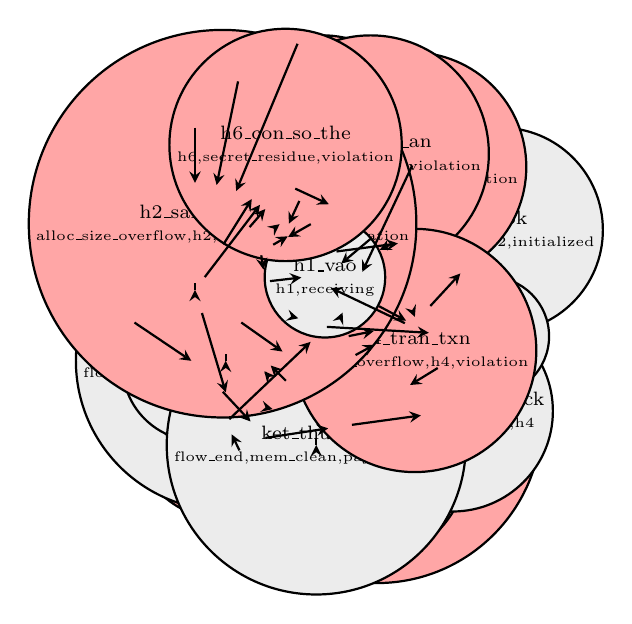
\begin{tikzpicture}[
  every node/.style={draw, circle, inner sep=2pt,
      minimum size=8mm, align=center, font=\scriptsize},
  ->, >=stealth, thick, auto
]
  \node[fill=red!35] (nd_h3_tran_so) at (-0.07,1.98) {h3\_tran\_so\\{\tiny h3,int\_overflow,violation}};
  \node[fill=red!35] (nd_h3_so_am) at (0.90,0.43) {h3\_so\_am\\{\tiny h3,negative\_amount,violation}};
  \node[fill=red!35] (nd_h6_double_free) at (-1.20,-1.47) {h6\_double\_free\\{\tiny double\_free,h6,violation}};
  \node[fill=gray!15] (nd_h2_vao) at (-0.70,0.51) {h2\_vao\\{\tiny allocating,h2}};
  \node[fill=red!35] (nd_h5_format_string) at (0.59,1.44) {h5\_format\_string\\{\tiny format\_string,h5,violation}};
  \node[fill=red!35] (nd_h2_doc_rac) at (-1.41,1.44) {h2\_doc\_rac\\{\tiny h2,uninit\_read,violation}};
  \node[fill=gray!15] (nd_h1_ok) at (1.67,-0.62) {h1\_ok\\{\tiny h1,input\_ok}};
  \node[fill=gray!15] (nd_h6_cb_giu) at (-0.78,-1.75) {h6\_cb\_giu\\{\tiny cb\_locked,h6}};
  \node[fill=gray!15] (nd_ket_thuc_tu_choi) at (-1.29,-0.77) {ket\_thuc\_tu\_choi\\{\tiny flow\_end,input\_rejected,mem\_clean}};
  \node[fill=gray!15] (nd_h6_phien_ranh) at (0.20,-1.60) {h6\_phien\_ranh\\{\tiny h6,sess\_free}};
  \node[fill=red!35] (nd_h1_tran_1_byte) at (0.63,-1.50) {h1\_tran\_1\_byte\\{\tiny buffer\_overflow,h1,off\_by\_one,violation}};
  \node[fill=red!35] (nd_h6_tranh_chap) at (0.22,-0.12) {h6\_tranh\_chap\\{\tiny cb\_locked,h6,race,to\_locked,violation}};
  \node[fill=gray!15] (nd_h4_vao) at (0.66,0.92) {h4\_vao\\{\tiny callback\_received,h4}};
  \node[fill=gray!15] (nd_dung_khong_an_toan) at (-1.68,0.13) {dung\_khong\_an\_toan\\{\tiny unsafe\_halt}};
  \node[fill=red!35] (nd_h3_chia_0) at (0.44,-1.99) {h3\_chia\_0\\{\tiny div\_by\_zero,h3,violation}};
  \node[fill=gray!15] (nd_h4_tu_choi_callback) at (1.59,-1.41) {h4\_tu\_choi\_callback\\{\tiny callback\_rejected,h4}};
  \node[fill=gray!15] (nd_h4_ok) at (-1.02,1.70) {h4\_ok\\{\tiny callback\_verified,h4}};
  \node[fill=gray!15] (nd_h2_ok) at (2.20,0.89) {h2\_ok\\{\tiny allocated,h2,initialized}};
  \node[fill=gray!15] (nd_h3_ok) at (-0.16,-0.98) {h3\_ok\\{\tiny amount\_ok,h3}};
  \node[fill=gray!15] (nd_h5_ok) at (2.06,-0.46) {h5\_ok\\{\tiny h5,log\_freed}};
  \node[fill=gray!15] (nd_h5_vao) at (-0.70,-0.30) {h5\_vao\\{\tiny h5,logging}};
  \node[fill=red!35] (nd_h2_null) at (-1.68,0.91) {h2\_null\\{\tiny h2,null\_deref,violation}};
  \node[fill=red!35] (nd_h1_tran_bo_dem) at (-0.61,1.53) {h1\_tran\_bo\_dem\\{\tiny buffer\_overflow,h1,violation}};
  \node[fill=blue!25] (nd_start) at (1.37,0.99) {start\\{\tiny safe,start}};
  \node[fill=red!35] (nd_h5_ro_ri) at (0.04,-1.89) {h5\_ro\_ri\\{\tiny h5,mem\_leak,violation}};
  \node[fill=gray!15] (nd_h3_vao) at (1.11,-0.29) {h3\_vao\\{\tiny computing,h3}};
  \node[fill=red!35] (nd_h6_uaf) at (1.07,1.69) {h6\_uaf\\{\tiny h6,use\_after\_free,violation}};
  \node[fill=red!35] (nd_h4_nhanh_an) at (0.55,1.86) {h4\_nhanh\_an\\{\tiny h4,hidden\_bypass,violation}};
  \node[fill=gray!15] (nd_h6_to_giu) at (-1.46,-1.20) {h6\_to\_giu\\{\tiny h6,to\_locked}};
  \node[fill=gray!15] (nd_h6_giai_phong) at (-1.64,-0.83) {h6\_giai\_phong\\{\tiny h6,releasing}};
  \node[fill=gray!15] (nd_ket_thuc_ok) at (-0.14,-1.84) {ket\_thuc\_ok\\{\tiny flow\_end,mem\_clean,payment\_done}};
  \node[fill=red!35] (nd_h4_tran_txn) at (1.11,-0.64) {h4\_tran\_txn\\{\tiny buffer\_overflow,h4,violation}};
  \node[fill=red!35] (nd_h2_sai_kich_thuoc) at (-1.33,0.97) {h2\_sai\_kich\_thuoc\\{\tiny alloc\_size\_overflow,h2,heap\_overflow,violation}};
  \node[fill=gray!15] (nd_h1_vao) at (-0.03,0.29) {h1\_vao\\{\tiny h1,receiving}};
  \node[fill=red!35] (nd_h6_con_so_the) at (-0.53,1.97) {h6\_con\_so\_the\\{\tiny h6,secret\_residue,violation}};
  \draw (nd_h3_tran_so) -- (nd_dung_khong_an_toan);
  \draw (nd_h3_so_am) -- (nd_dung_khong_an_toan);
  \draw (nd_h6_double_free) -- (nd_dung_khong_an_toan);
  \draw (nd_h2_vao) -- (nd_h2_ok);
  \draw (nd_h2_vao) -- (nd_ket_thuc_tu_choi);
  \draw (nd_h5_format_string) -- (nd_dung_khong_an_toan);
  \draw (nd_h2_doc_rac) -- (nd_dung_khong_an_toan);
  \draw (nd_h1_ok) -- (nd_h2_vao);
  \draw (nd_h6_cb_giu) -- (nd_h6_giai_phong);
  \draw (nd_ket_thuc_tu_choi) -- (nd_ket_thuc_tu_choi);
  \draw (nd_h6_phien_ranh) -- (nd_h6_cb_giu);
  \draw (nd_h6_phien_ranh) -- (nd_h6_to_giu);
  \draw (nd_h1_tran_1_byte) -- (nd_dung_khong_an_toan);
  \draw (nd_h6_tranh_chap) -- (nd_h6_double_free);
  \draw (nd_h6_tranh_chap) -- (nd_h6_uaf);
  \draw (nd_h4_vao) -- (nd_h4_ok);
  \draw (nd_h4_vao) -- (nd_h4_tu_choi_callback);
  \draw (nd_dung_khong_an_toan) -- (nd_dung_khong_an_toan);
  \draw (nd_h3_chia_0) -- (nd_dung_khong_an_toan);
  \draw (nd_h4_tu_choi_callback) -- (nd_h6_phien_ranh);
  \draw (nd_h4_ok) -- (nd_h5_vao);
  \draw (nd_h2_ok) -- (nd_h3_vao);
  \draw (nd_h3_ok) -- (nd_h4_vao);
  \draw (nd_h5_ok) -- (nd_h6_phien_ranh);
  \draw (nd_h5_vao) -- (nd_h5_ok);
  \draw (nd_h2_null) -- (nd_dung_khong_an_toan);
  \draw (nd_h1_tran_bo_dem) -- (nd_dung_khong_an_toan);
  \draw (nd_start) -- (nd_h1_vao);
  \draw (nd_h5_ro_ri) -- (nd_dung_khong_an_toan);
  \draw (nd_h3_vao) -- (nd_ket_thuc_tu_choi);
  \draw (nd_h3_vao) -- (nd_h3_ok);
  \draw (nd_h6_uaf) -- (nd_dung_khong_an_toan);
  \draw (nd_h4_nhanh_an) -- (nd_dung_khong_an_toan);
  \draw (nd_h6_to_giu) -- (nd_h6_giai_phong);
  \draw (nd_h6_giai_phong) -- (nd_ket_thuc_ok);
  \draw (nd_ket_thuc_ok) -- (nd_ket_thuc_ok);
  \draw (nd_h4_tran_txn) -- (nd_dung_khong_an_toan);
  \draw (nd_h2_sai_kich_thuoc) -- (nd_dung_khong_an_toan);
  \draw (nd_h1_vao) -- (nd_h1_ok);
  \draw (nd_h1_vao) -- (nd_ket_thuc_tu_choi);
  \draw (nd_h6_con_so_the) -- (nd_dung_khong_an_toan);
\end{tikzpicture}

% M1-v1b: bản sửa của nhóm — buf[17] + strnlen + từ chối
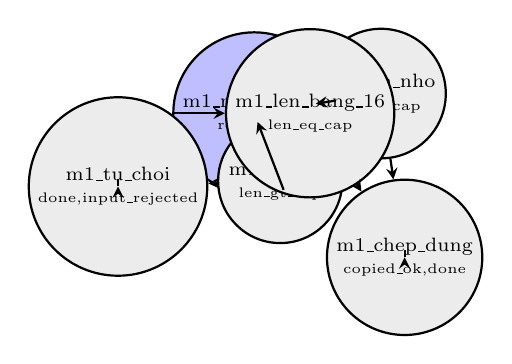
\begin{tikzpicture}[
  every node/.style={draw, circle, inner sep=2pt,
      minimum size=8mm, align=center, font=\scriptsize},
  ->, >=stealth, thick, auto
]
  \node[fill=gray!15] (nd_m1_len_nho) at (1.14,0.81) {m1\_len\_nho\\{\tiny len\_lt\_cap}};
  \node[fill=gray!15] (nd_m1_chep_dung) at (1.44,-1.27) {m1\_chep\_dung\\{\tiny copied\_ok,done}};
  \node[fill=blue!25] (nd_m1_nhan_chuoi) at (-0.47,0.56) {m1\_nhan\_chuoi\\{\tiny receiving}};
  \node[fill=gray!15] (nd_m1_tu_choi) at (-2.20,-0.37) {m1\_tu\_choi\\{\tiny done,input\_rejected}};
  \node[fill=gray!15] (nd_m1_len_lon) at (-0.14,-0.30) {m1\_len\_lon\\{\tiny len\_gt\_cap}};
  \node[fill=gray!15] (nd_m1_len_bang_16) at (0.24,0.56) {m1\_len\_bang\_16\\{\tiny len\_eq\_cap}};
  \draw (nd_m1_len_nho) -- (nd_m1_chep_dung);
  \draw (nd_m1_chep_dung) -- (nd_m1_chep_dung);
  \draw (nd_m1_nhan_chuoi) -- (nd_m1_len_bang_16);
  \draw (nd_m1_nhan_chuoi) -- (nd_m1_len_nho);
  \draw (nd_m1_nhan_chuoi) -- (nd_m1_len_lon);
  \draw (nd_m1_tu_choi) -- (nd_m1_tu_choi);
  \draw (nd_m1_len_lon) -- (nd_m1_tu_choi);
  \draw (nd_m1_len_bang_16) -- (nd_m1_chep_dung);
\end{tikzpicture}

% M2-v1: kiểm tra n, calloc, kiểm tra NULL
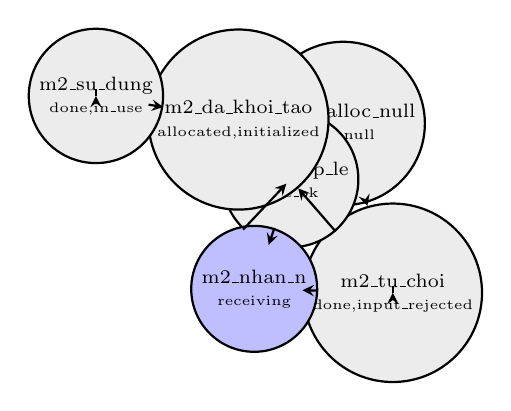
\begin{tikzpicture}[
  every node/.style={draw, circle, inner sep=2pt,
      minimum size=8mm, align=center, font=\scriptsize},
  ->, >=stealth, thick, auto
]
  \node[fill=gray!15] (nd_m2_malloc_null) at (0.94,0.76) {m2\_malloc\_null\\{\tiny ptr\_null}};
  \node[fill=gray!15] (nd_m2_tu_choi) at (1.57,-1.39) {m2\_tu\_choi\\{\tiny done,input\_rejected}};
  \node[fill=gray!15] (nd_m2_n_hop_le) at (0.27,0.05) {m2\_n\_hop\_le\\{\tiny size\_ok}};
  \node[fill=blue!25] (nd_m2_nhan_n) at (-0.19,-1.34) {m2\_nhan\_n\\{\tiny receiving}};
  \node[fill=gray!15] (nd_m2_da_khoi_tao) at (-0.39,0.81) {m2\_da\_khoi\_tao\\{\tiny allocated,initialized}};
  \node[fill=gray!15] (nd_m2_su_dung) at (-2.20,1.11) {m2\_su\_dung\\{\tiny done,in\_use}};
  \draw (nd_m2_malloc_null) -- (nd_m2_tu_choi);
  \draw (nd_m2_tu_choi) -- (nd_m2_tu_choi);
  \draw (nd_m2_n_hop_le) -- (nd_m2_malloc_null);
  \draw (nd_m2_n_hop_le) -- (nd_m2_da_khoi_tao);
  \draw (nd_m2_nhan_n) -- (nd_m2_tu_choi);
  \draw (nd_m2_nhan_n) -- (nd_m2_n_hop_le);
  \draw (nd_m2_da_khoi_tao) -- (nd_m2_su_dung);
  \draw (nd_m2_su_dung) -- (nd_m2_su_dung);
\end{tikzpicture}

% M3-v1: kiểm tra miền + int64 + hạn mức
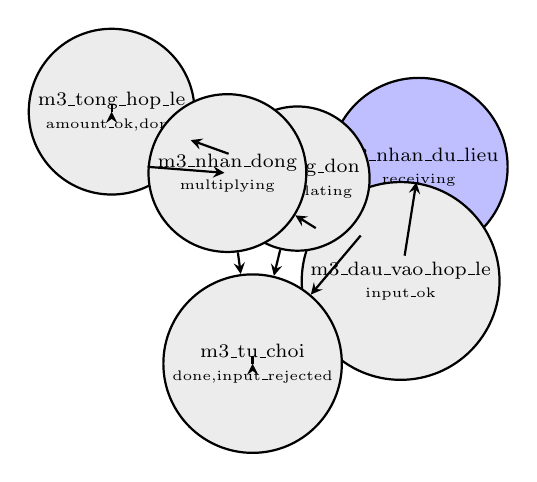
\begin{tikzpicture}[
  every node/.style={draw, circle, inner sep=2pt,
      minimum size=8mm, align=center, font=\scriptsize},
  ->, >=stealth, thick, auto
]
  \node[fill=blue!25] (nd_m3_nhan_du_lieu) at (1.70,0.58) {m3\_nhan\_du\_lieu\\{\tiny receiving}};
  \node[fill=gray!15] (nd_m3_dau_vao_hop_le) at (1.47,-0.87) {m3\_dau\_vao\_hop\_le\\{\tiny input\_ok}};
  \node[fill=gray!15] (nd_m3_tu_choi) at (-0.41,-1.92) {m3\_tu\_choi\\{\tiny done,input\_rejected}};
  \node[fill=gray!15] (nd_m3_tong_hop_le) at (-2.20,1.28) {m3\_tong\_hop\_le\\{\tiny amount\_ok,done}};
  \node[fill=gray!15] (nd_m3_cong_don) at (0.16,0.43) {m3\_cong\_don\\{\tiny accumulating}};
  \node[fill=gray!15] (nd_m3_nhan_dong) at (-0.73,0.50) {m3\_nhan\_dong\\{\tiny multiplying}};
  \draw (nd_m3_nhan_du_lieu) -- (nd_m3_tu_choi);
  \draw (nd_m3_nhan_du_lieu) -- (nd_m3_dau_vao_hop_le);
  \draw (nd_m3_dau_vao_hop_le) -- (nd_m3_nhan_dong);
  \draw (nd_m3_tu_choi) -- (nd_m3_tu_choi);
  \draw (nd_m3_tong_hop_le) -- (nd_m3_tong_hop_le);
  \draw (nd_m3_cong_don) -- (nd_m3_tu_choi);
  \draw (nd_m3_cong_don) -- (nd_m3_tong_hop_le);
  \draw (nd_m3_nhan_dong) -- (nd_m3_cong_don);
  \draw (nd_m3_nhan_dong) -- (nd_m3_tu_choi);
\end{tikzpicture}

% M4-v1: kiểm tra độ dài, xóa nhánh ẩn
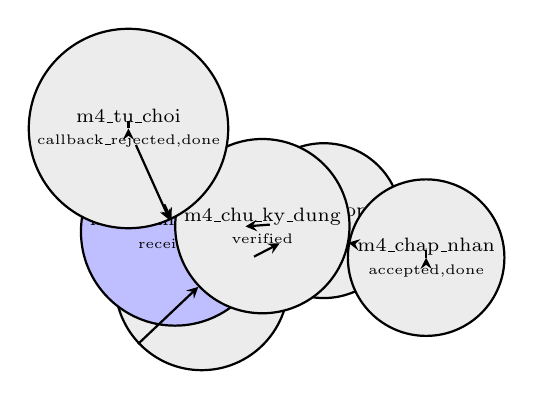
\begin{tikzpicture}[
  every node/.style={draw, circle, inner sep=2pt,
      minimum size=8mm, align=center, font=\scriptsize},
  ->, >=stealth, thick, auto
]
  \node[fill=gray!15] (nd_m4_txn_hop_le) at (0.90,0.05) {m4\_txn\_hop\_le\\{\tiny len\_ok}};
  \node[fill=gray!15] (nd_m4_kiem_chu_ky) at (-0.65,-0.75) {m4\_kiem\_chu\_ky\\{\tiny verifying}};
  \node[fill=blue!25] (nd_m4_nhan_callback) at (-0.99,-0.09) {m4\_nhan\_callback\\{\tiny receiving}};
  \node[fill=gray!15] (nd_m4_chu_ky_dung) at (0.12,-0.02) {m4\_chu\_ky\_dung\\{\tiny verified}};
  \node[fill=gray!15] (nd_m4_chap_nhan) at (2.20,-0.42) {m4\_chap\_nhan\\{\tiny accepted,done}};
  \node[fill=gray!15] (nd_m4_tu_choi) at (-1.58,1.22) {m4\_tu\_choi\\{\tiny callback\_rejected,done}};
  \draw (nd_m4_txn_hop_le) -- (nd_m4_kiem_chu_ky);
  \draw (nd_m4_kiem_chu_ky) -- (nd_m4_tu_choi);
  \draw (nd_m4_kiem_chu_ky) -- (nd_m4_chu_ky_dung);
  \draw (nd_m4_nhan_callback) -- (nd_m4_txn_hop_le);
  \draw (nd_m4_nhan_callback) -- (nd_m4_tu_choi);
  \draw (nd_m4_chu_ky_dung) -- (nd_m4_chap_nhan);
  \draw (nd_m4_chap_nhan) -- (nd_m4_chap_nhan);
  \draw (nd_m4_tu_choi) -- (nd_m4_tu_choi);
\end{tikzpicture}

% M5-v1: printf("%s") + goto cleanup
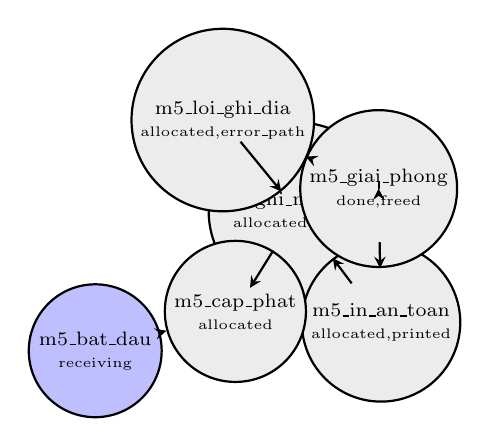
\begin{tikzpicture}[
  every node/.style={draw, circle, inner sep=2pt,
      minimum size=8mm, align=center, font=\scriptsize},
  ->, >=stealth, thick, auto
]
  \node[fill=gray!15] (nd_m5_ghi_noi_dung) at (0.37,0.50) {m5\_ghi\_noi\_dung\\{\tiny allocated,in\_use}};
  \node[fill=gray!15] (nd_m5_in_an_toan) at (1.43,-0.91) {m5\_in\_an\_toan\\{\tiny allocated,printed}};
  \node[fill=gray!15] (nd_m5_cap_phat) at (-0.42,-0.77) {m5\_cap\_phat\\{\tiny allocated}};
  \node[fill=blue!25] (nd_m5_bat_dau) at (-2.20,-1.27) {m5\_bat\_dau\\{\tiny receiving}};
  \node[fill=gray!15] (nd_m5_giai_phong) at (1.40,0.79) {m5\_giai\_phong\\{\tiny done,freed}};
  \node[fill=gray!15] (nd_m5_loi_ghi_dia) at (-0.58,1.66) {m5\_loi\_ghi\_dia\\{\tiny allocated,error\_path}};
  \draw (nd_m5_ghi_noi_dung) -- (nd_m5_loi_ghi_dia);
  \draw (nd_m5_ghi_noi_dung) -- (nd_m5_in_an_toan);
  \draw (nd_m5_in_an_toan) -- (nd_m5_giai_phong);
  \draw (nd_m5_cap_phat) -- (nd_m5_ghi_noi_dung);
  \draw (nd_m5_bat_dau) -- (nd_m5_cap_phat);
  \draw (nd_m5_giai_phong) -- (nd_m5_giai_phong);
  \draw (nd_m5_loi_ghi_dia) -- (nd_m5_giai_phong);
\end{tikzpicture}

% M6-v1: mutex + status CLOSED + explicit_bzero
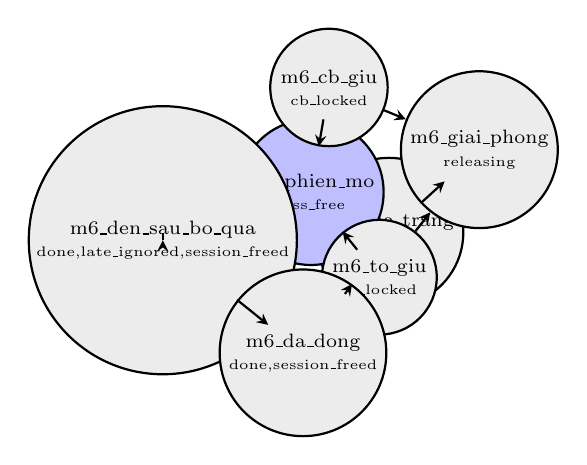
\begin{tikzpicture}[
  every node/.style={draw, circle, inner sep=2pt,
      minimum size=8mm, align=center, font=\scriptsize},
  ->, >=stealth, thick, auto
]
  \node[fill=gray!15] (nd_m6_xoa_trang) at (0.67,-0.17) {m6\_xoa\_trang\\{\tiny wiped}};
  \node[fill=blue!25] (nd_m6_phien_mo) at (-0.32,0.34) {m6\_phien\_mo\\{\tiny sess\_free}};
  \node[fill=gray!15] (nd_m6_to_giu) at (0.55,-0.74) {m6\_to\_giu\\{\tiny to\_locked}};
  \node[fill=gray!15] (nd_m6_den_sau_bo_qua) at (-2.20,-0.27) {m6\_den\_sau\_bo\_qua\\{\tiny done,late\_ignored,session\_freed}};
  \node[fill=gray!15] (nd_m6_giai_phong) at (1.82,0.88) {m6\_giai\_phong\\{\tiny releasing}};
  \node[fill=gray!15] (nd_m6_cb_giu) at (-0.09,1.67) {m6\_cb\_giu\\{\tiny cb\_locked}};
  \node[fill=gray!15] (nd_m6_da_dong) at (-0.42,-1.70) {m6\_da\_dong\\{\tiny done,session\_freed}};
  \draw (nd_m6_xoa_trang) -- (nd_m6_da_dong);
  \draw (nd_m6_phien_mo) -- (nd_m6_to_giu);
  \draw (nd_m6_phien_mo) -- (nd_m6_cb_giu);
  \draw (nd_m6_to_giu) -- (nd_m6_giai_phong);
  \draw (nd_m6_den_sau_bo_qua) -- (nd_m6_den_sau_bo_qua);
  \draw (nd_m6_giai_phong) -- (nd_m6_xoa_trang);
  \draw (nd_m6_cb_giu) -- (nd_m6_giai_phong);
  \draw (nd_m6_da_dong) -- (nd_m6_den_sau_bo_qua);
\end{tikzpicture}